\chapter{Introduction}
% First chapter.
% \section{Background}

Belt sorting is a type of technology that can automatically separate different types of materials or filter out the unaccepted products from the material flow with conveyor belts. This technology has been widely used in different industry areas, such as mining, recycling \cite{pfaff2015tracksort} and food processing \cite{edwards2004detecting}. Belt sorting enables an automatic process of sorting that significantly saves time, human resources, cost as well as energy \cite{zsifkovits2020state}.

Optical sorting sorts bulk materials according to the optical features of the particles. Compared with the other sorting methods based on the physical properties, optical sorting is less limited from the type of materials and able to sort the materials in a non-destructive way. An optical belt sorting system usually comprises four parts: the feed system, the optical system, the data processing system, and the separation system, as illustrated in Figure \ref{belt sort system old} \cite{edwards2004detecting}. Conventional optical belt sorting systems use a line camera at the end of the conveyor belt to detect the particles. In this case, each particle is observed only once and assumed as flying straightly in the transport direction and reaching the separator after a fixed delay \cite{wotruba2008stand}. However, this simple motion model is inadequate for predicting the motion of the particles, and the sorting accuracy is therefore limited, as shown in Figure \ref{line camera error}.

\begin{figure}[htb]
\centering
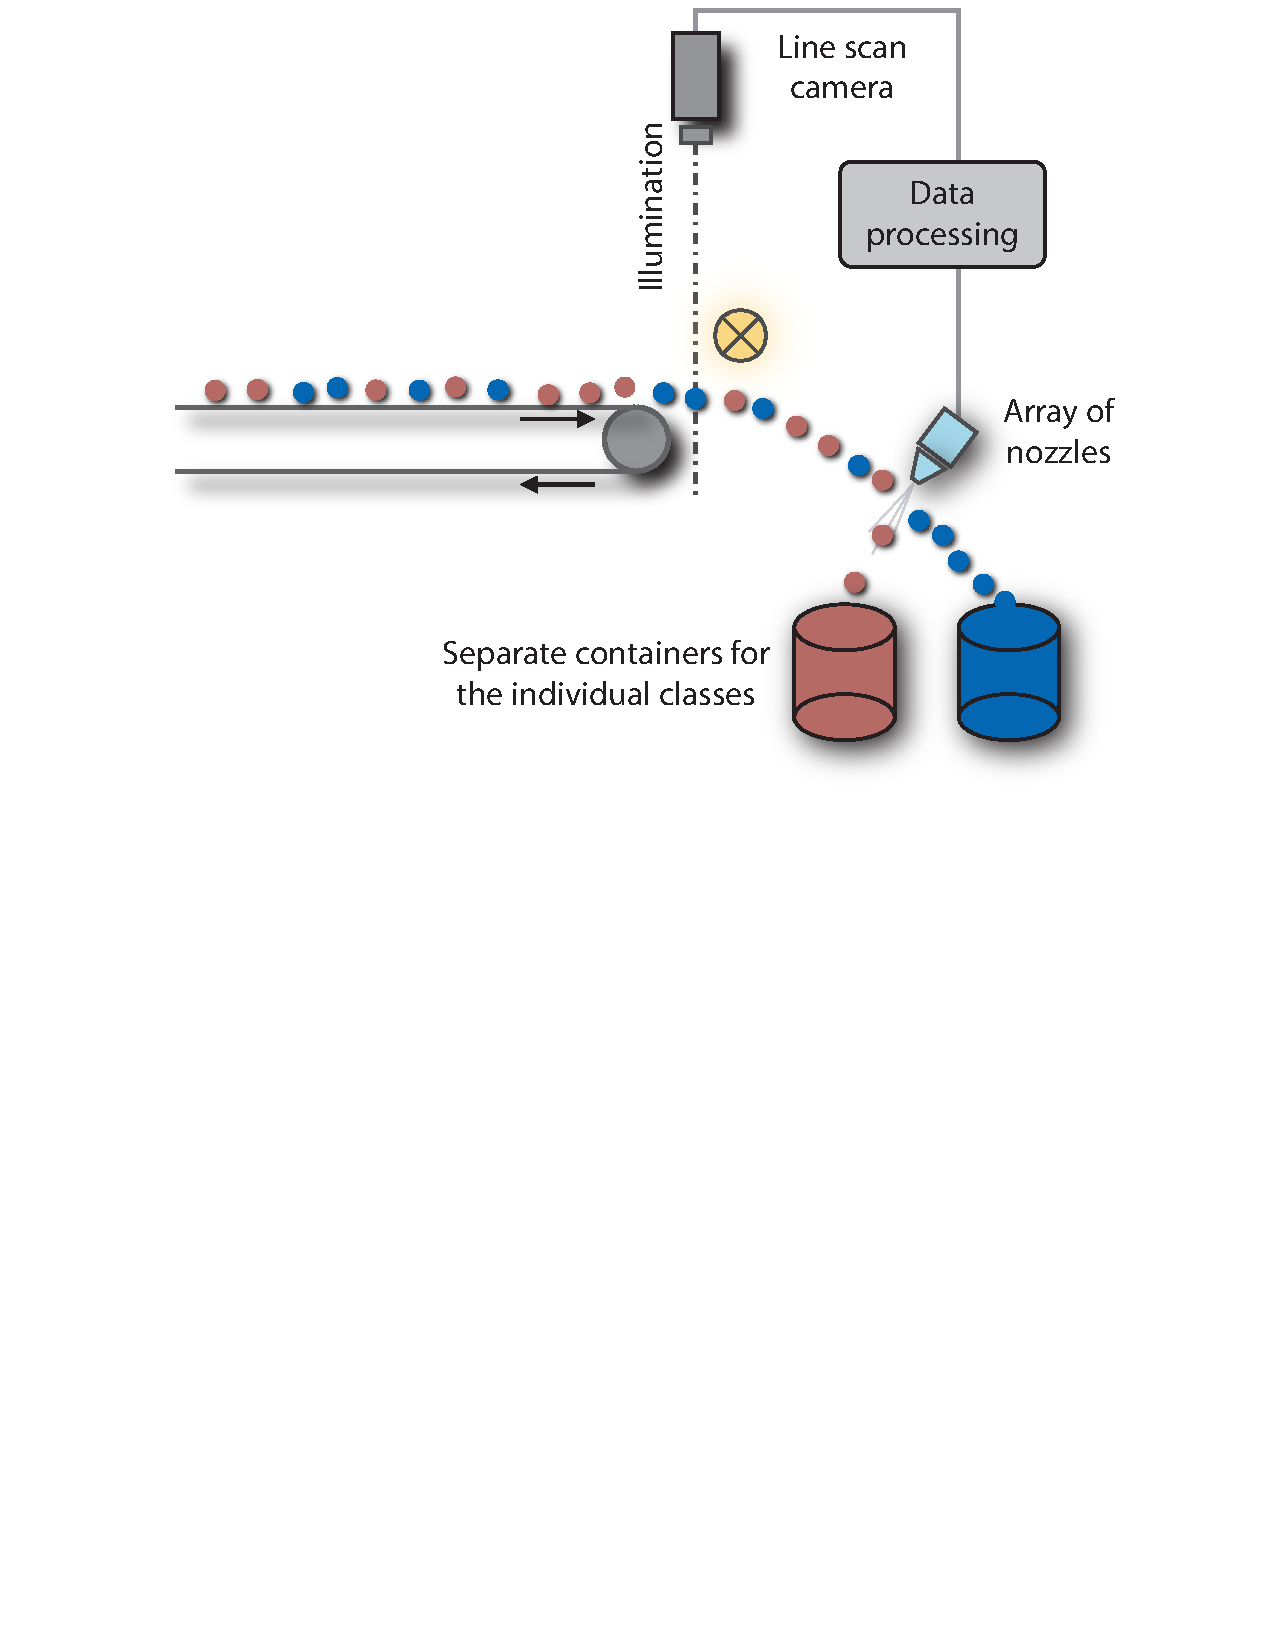
\includegraphics[width=0.5\textwidth]{figures/sort system old.pdf}
\caption{Structure of a conventional optical belt sorting system with line scan camera. In our recent research, the line scan camera has been replaced with a area scan camera. The figure is adapted from \cite{pfaff2017improving}.}
\label{belt sort system old}
\end{figure}

\begin{figure}[htb]
\centering
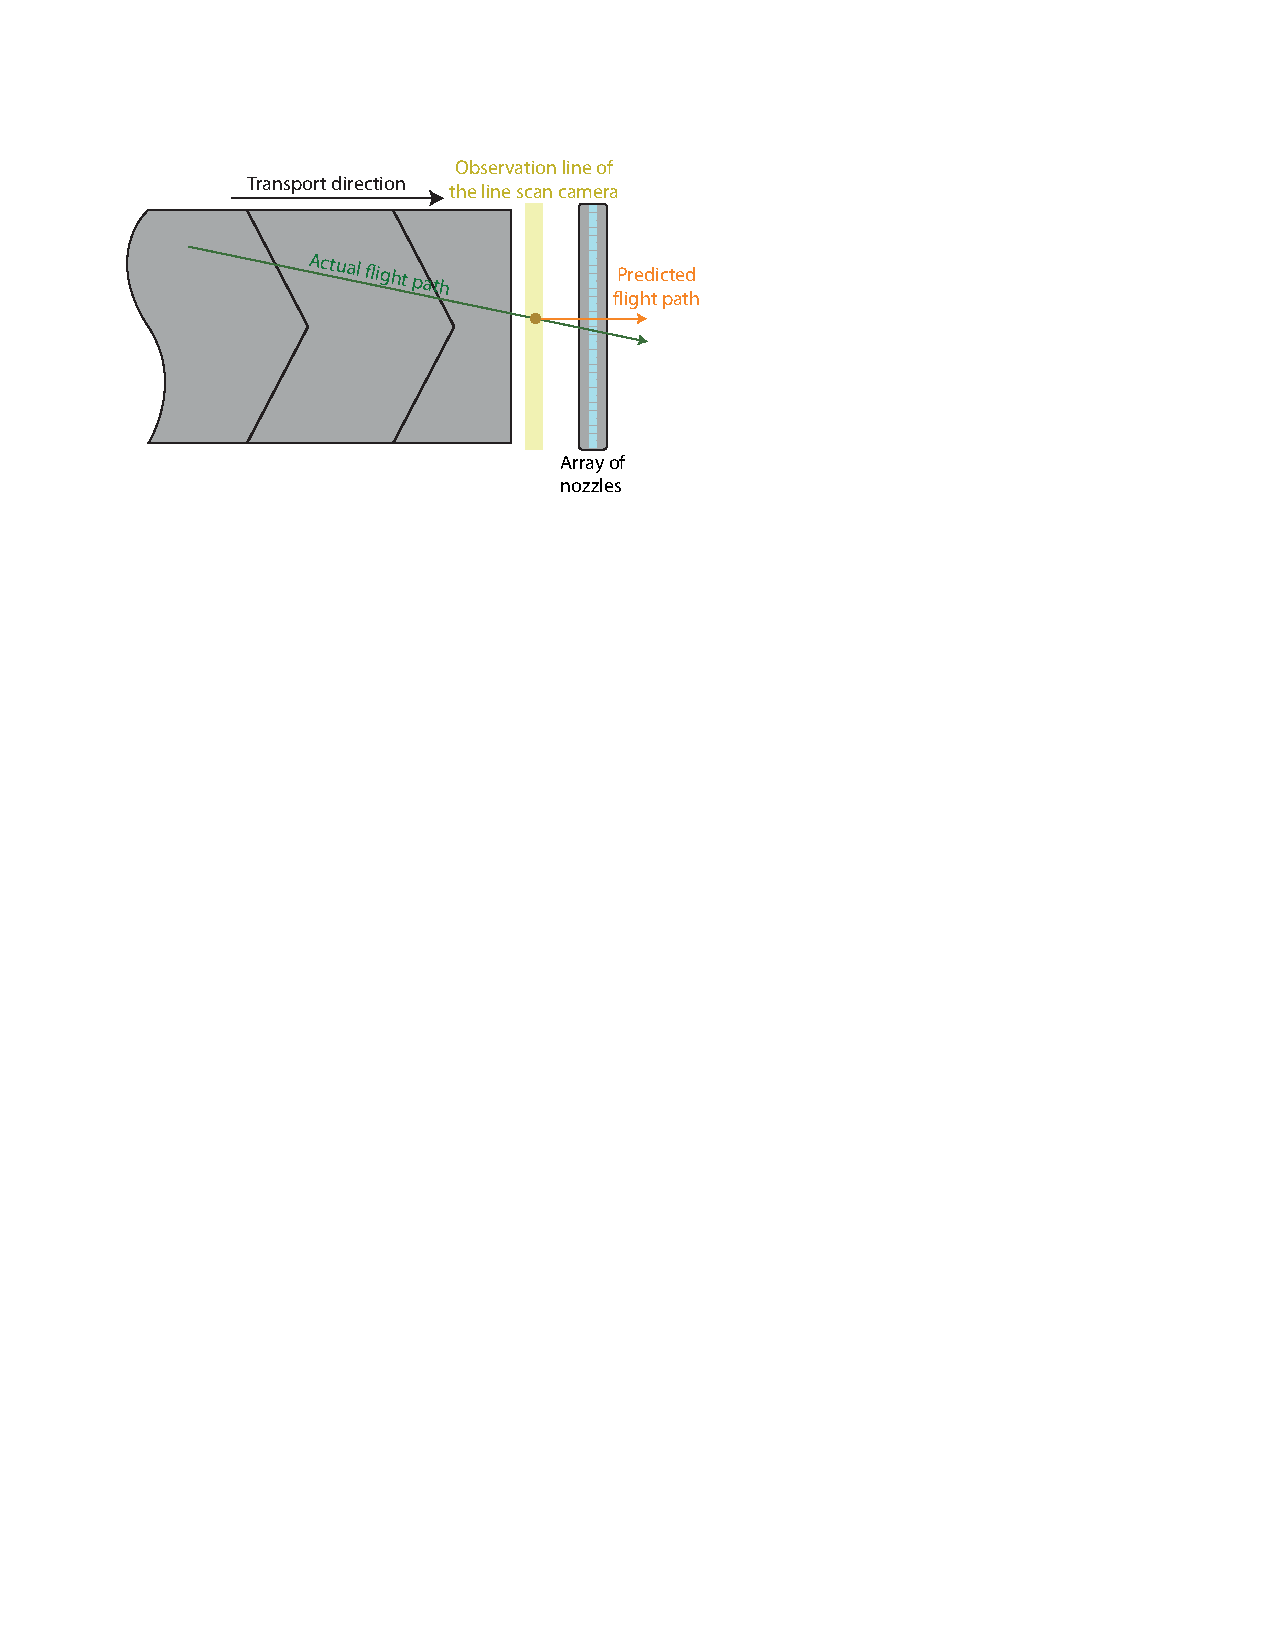
\includegraphics[width=0.5\textwidth]{figures/line camera.pdf}
\caption{Illustration that the prediction of the particle motion can be imprecise when assuming a motion straight along the transport direction \cite{pfaff2019multitarget}.}
\label{line camera error}
\end{figure}

In order to overcome the drawbacks of the belt sorter with line cameras, Pfaff et al. \cite{pfaff2019multitarget} replaced the line cameras with area cameras. The area camera takes pictures containing multiple particles, and the particles can be observed from the camera in multiple frames. With the area camera, we are able to perform a multitarget tracking of the particles on the belt, with which the more precise information of the particles, such as velocity and even acceleration, can be obtained. Then with the motion model for the prediction to the separator nozzles, the motion of the particles can be more accurately predicted.

\section{Motivation and Contribution}

The multitarget tracking algorithm is composed of the single-target motion prediction part that estimates the motion of particles and the association part that assigns the measurements to each particle, as shown in Figure \ref{tracking system simple}. In both parts, the algorithm needs different hyperparameters that need to be tuned before we are able to run the algorithm properly, such as the variance term in Kalman filter and the penalty term in the association matrix. Choosing appropriate parameters for different bulk materials can significantly improve the performance of the multitarget tracking algorithm.

\begin{figure}[htb]
\centering
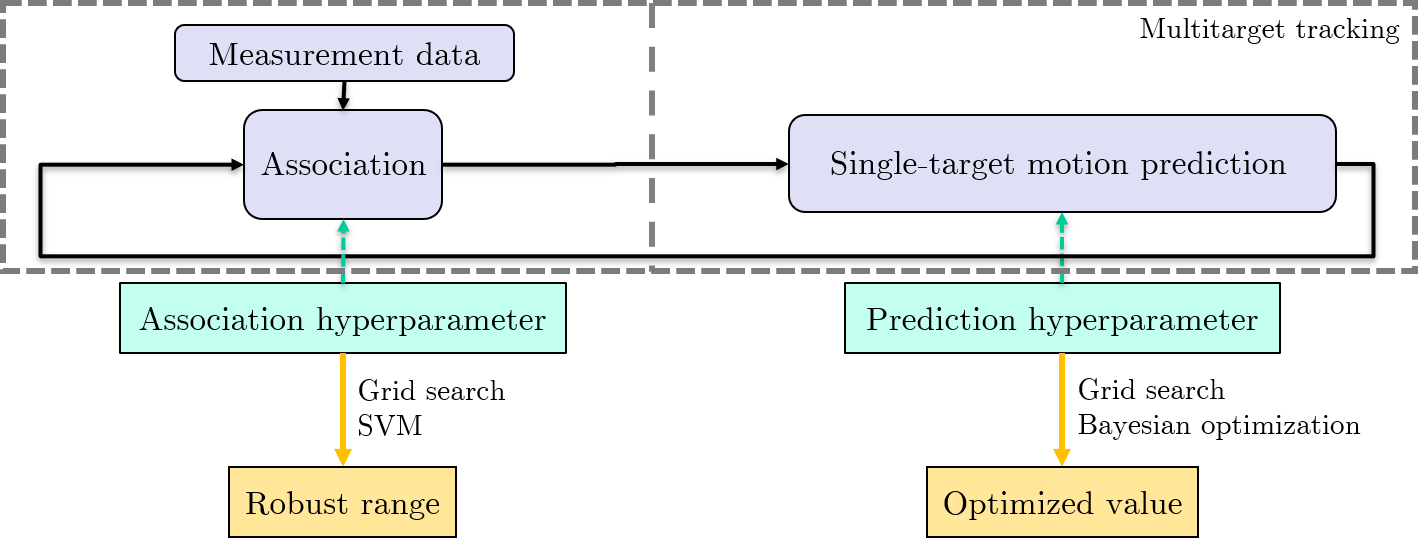
\includegraphics[width=0.9\textwidth]{figures/tracking system simple.png}
\caption{Structure of the multitarget tracking algorithm, including the single-target motion prediction part and the association part, which contain different hyperparameters. These hyperparameters are optimized with different methods in this thesis.}
\label{tracking system simple}
\end{figure}

The optimal value of the hyperparameters depend on many properties of the material, such as the shapes and sizes of the particles. However, the hyperparameters have been manually determined so far and lack a systematic method for finding the optimal values. These manually determined values of hyperparameters are not adaptive to the different materials or dynamical situations in sorting. Therefore, the hyperparameters need to be optimized, and the optimization methods should be generalized for all kinds of materials.


In this thesis, the hyperparameters in both parts of the tracking algorithm are optimized with different methods. In the single-target motion prediction part, the hyperparameters are optimized with grid search and Bayesian optimization. The prediction error is lowered with the optimized hyperparameters, and the difference of the optimized hyperparameter values between materials is discussed. The robust ranges of the association hyperparameters are determined with grid search and SVMs. The determination criteria for the robust range based on the average prediction error and particle density are also discussed.

\section{Thesis Outline}


In Chapter 2, we introduce the theoretical basis needed in this thesis, including the basic ideas of the tracking algorithm and optimization algorithms. These contents can give us the initial knowledge of the multitarget tracking system we work on and the optimization tools we have. Chapter 3 presents more details of the implementation of the multitarget tracking algorithm. All the hyperparameters for the optimization are also listed in this chapter. Chapter 4 makes an introduction of the datasets used in the thesis. Chapter 5 introduces the method and their settings for the optimization works in this thesis. The evaluation criteria of the prediction and association performance is also presented in this chapter. Chapter 6 shows the results of all experiments, including the optimized values for hyperparameters and the effect of optimizations. Some explanations and discussions are also given after the results. The thesis ends with Chapter 7, which gives the conclusion of this thesis as well as some suggestions and outlooks for future researches.




% s. The first half of this chapter presents the initial knowledge of the tracking algorithm, including the system model, Kalman filter, motion models and multitarget tracking. The important algorithms for optimization and classification are reviewed in the second half of this chapter. The optimization algorithms are explained briefly in Section 2.3. Then the method of grid search and Bayesian optimization is in detail explained. In Section 2.4, the principle of SVM is explained. In the following section, overfitting and the methods for avoiding it are discussed.

% Chapter 3 presents more detailed knowledge of the \textit{TrackSort} algorithm. In the first two sections, the basics of the traditional belt sorting system as well as the development of the \textit{TableSort}-System and the \textit{TrackSort} algorithm are presented. In Section 3.3, the \textit{TrackSort} algorithm is more in detail explained, including the motion models used for tracking and the methods for data association and track management.

% Chapter 4 focuses on the datasets used in the thesis. Four types of datasets are introduced, namely the datasets from single real materials, the datasets from mixed real materials, the DEM datasets and the artificial datasets.

% Chapter 5 introduces the method for the optimization works in this thesis. In Section 5.1, the evaluation metrics for motion prediction and association are first presented. Then in Section 5.2 the methods and settings for optimization of the prediction hyperparameters are depicted. In Section 5.3, the concept of the robust range is introduced, then the settings and the process of the training of SVMs are in detail explained.

% Chapter 6 shows the results of all experiments. The effect of the prediction hyperparameters is shown in Section 6.1, then the optimized value for the test dataset and more datasets are presented in the following subsections. In Section 6.2, the result of the robust range for association hyperparameters is explained.

% The thesis ends with Chapter 7, which gives the conclusion of this thesis. In this chapter, some suggestions and outlooks for future research are also raised.